\section{Klassendiagramm}
\label{sec:klassendiagramm}

Da die Applikation keinerlei BenutzerInneninteraktion vorsieht und auch kaum
Daten konsistent speichern noch in irgendeiner Form manipulieren muss, fällt das
Klassendiagramm sehr knapp aus.

Die Klasse Konfiguration entählt alle Werte, die von der Applikation konsitent
(z.B. im lokalen Dateisystem) gespeichert werden sollen und die keiner anderen
Klasse logisch zugeordnet werden können.

Die Klasse Suchbegriff ist abstrakt. Sie definiert lediglich ein Attribut,
welches sie an die Klassen Suchwort und Suchsatz vererbt. Der Suchbegriff ist
also entweder ein Suchwort, oder ein Suchsatz. Dies hängt vom Rückgabewert und
somit von der Implementation der Server-Komponente ab, welche in dieser Arbeit
nicht spezifiziert wird.

Das Suchwort sowie der Suchsatz besitzen keine eigenen Attribute. Ihr einziges
Attribut erben sie vom Suchbegriff, nämlich den Text, welcher das Wort bzw.
den Satz für die Suchanfrage bei Google beinhaltet. Getrennt wurden die beiden
Klassen aus logischen Gründen, um bestmögliche Modifizierbarkeit zu
gewährleisten (siehe dazu die nichtfunktionalen Anforderungen im Pflichtenheft).

Die Klasse Suchergebnis steht in folgender Beziehung zum Suchbegriff: Jedes
Suchergebnis hat genau einen Suchbegriff, jeder Suchbegriff hat beliebig viele
Suchergebnisse.
\\[\intextsep]
\begin{minipage}{\linewidth}
\centering%
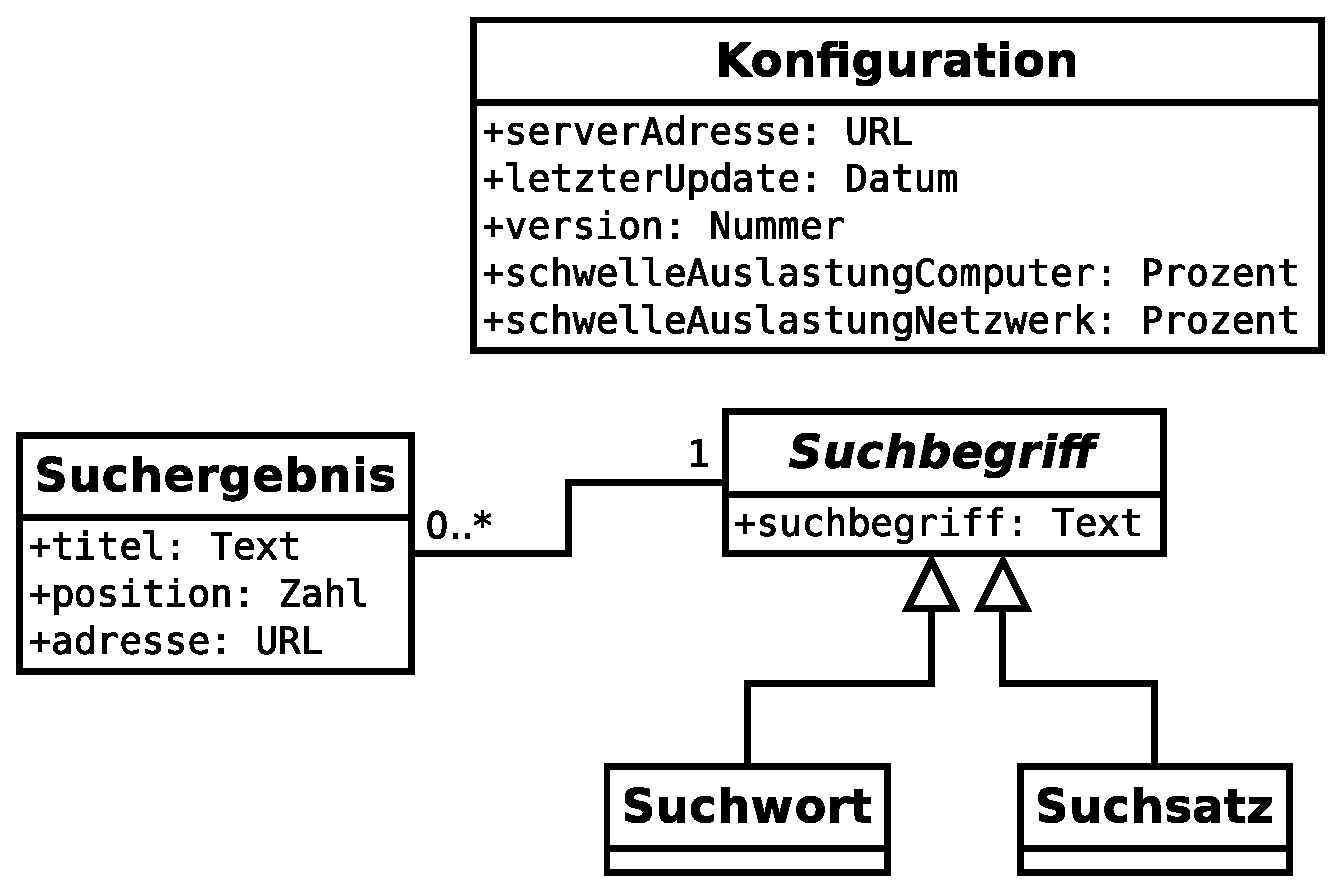
\includegraphics[scale=0.4,clip=]{img/klassendiagramm.eps}%
\figcaption{Klassendiagramm}%
\label{fig:klassendiagramm}%
\end{minipage}
